\documentclass[border=1mm]{standalone}
\usepackage{amsfonts,tikz,tikz-layers}
\usepackage{ccicons}
\usetikzlibrary{fadings,quotes, shapes,calc,decorations.markings}
\usetikzlibrary{patterns}
\usetikzlibrary{shadows.blur}
\usetikzlibrary{shapes,shapes.geometric,positioning, arrows, arrows.meta}
\usetikzlibrary{backgrounds}
\usetikzlibrary{decorations.text}
\definecolor{mblue}{HTML}{0077B5}

\begin{document}
\sffamily % Set the entire document to sans-serif font
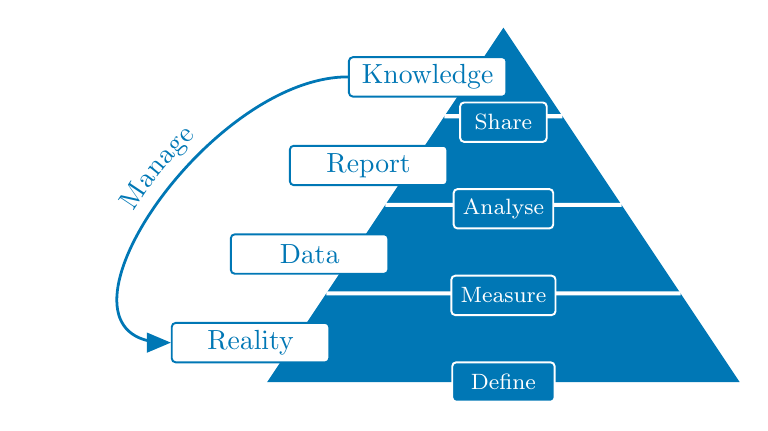
\begin{tikzpicture}[line width=.7pt]

  % Triangle
\fill[mblue] (0,0)--(6,0)-- coordinate[pos=.25] (p1) coordinate[pos=.5] (p2) coordinate[pos=.75] (p3) (3,4.5)-- coordinate[pos=.25] (n3) coordinate[pos=.5] (n2) coordinate[pos=.75] (n1) coordinate[pos=1] (n0) cycle;
\draw[white,line width=1.5pt] (n1)--(p1);
\draw[white,line width=1.5pt] (n2)--(p2);
\draw[white,line width=1.5pt] (n3)--(p3);

% Text boxes
\node[draw=mblue, minimum width=2cm,minimum height=.5cm, fill=white, shift={(.8,.5)}, rounded corners=.5mm, text=mblue, anchor=east,inner ysep=0pt] (kn) at (n3) {Knowledge};
\node[draw=mblue, minimum width=2cm,minimum height=.5cm, fill=white, shift={(.8,.5)}, rounded corners=.5mm, text=mblue, anchor=east, inner ysep=0pt] at (n2) {Report};
\node[draw=mblue, minimum width=2cm,minimum height=.5cm, fill=white, shift={(.8,.5)}, rounded corners=.5mm, text=mblue, anchor=east, inner ysep=0pt] at (n1) {Data};
\node[draw=mblue, minimum width=2cm,minimum height=.5cm, fill=white, shift={(.8,.5)}, rounded corners=.5mm, text=mblue, anchor=east, inner ysep=0pt] (re) at (n0) {Reality};

% Curved arrow
\begin{scope}[on behind layer]
\draw[mblue, triangle 45-, line width=1pt, 
    postaction={decorate, 
        decoration={text along path, text={Manage}, text align=center, raise=2mm, text color=mblue}}]
    ([xshift=0mm]re.west) 
    .. controls +(-1.8,0) and +(-1.8,0) .. 
    ([xshift=0mm]kn.west);
\end{scope}

% Action boxes
\node[draw=white, minimum width=1.3cm,minimum height=.5cm, fill=mblue, rounded corners=.5mm, text=white, anchor=center, inner ysep=0pt] 
    at (3, 0) {\footnotesize{Define}}; % Adjusted position for better centering
\node[draw=white, minimum width=1.1cm,minimum height=.5cm, fill=mblue, rounded corners=.5mm, text=white, anchor=center, inner ysep=0pt] 
    at (3, 1.1) {\footnotesize{Measure}}; % Adjusted position for better centering
\node[draw=white, minimum width=1.1cm,minimum height=.5cm, fill=mblue, rounded corners=.5mm, text=white, anchor=center, inner ysep=0pt] 
    at (3, 2.2) {\footnotesize{Analyse}}; % Adjusted position for better centering
\node[draw=white, minimum width=1.1cm,minimum height=.5cm, fill=mblue, rounded corners=.5mm, text=white, anchor=center, inner ysep=0pt] 
    at (3, 3.3) {\footnotesize{Share}}; % Adjusted position for better centering

\end{tikzpicture}
\end{document}
